\documentclass{beamer}

\usepackage{amsmath}
\usepackage{tabularx}
\usepackage{natbib}
\usepackage{verbatim}
\usepackage{listings}
\usepackage{tikz,xifthen}
\usepackage{booktabs}
\usepackage{eurosym}
\usepackage{graphicx}
\usetikzlibrary{shapes,arrows,positioning,shadows}
\usenavigationsymbolstemplate{}
\setbeamertemplate{caption}[numbered]



\newcommand{\bftt}[1]{\textbf{\texttt{#1}}}
\newcommand{\comments}[1]{{\color[HTML]{008080}\textit{\textbf{\texttt{#1}}}}}
\newcommand{\cmd}[1]{{\color[HTML]{008000}\bftt{#1}}}
\newcommand{\bs}{\char`\\}
\newcommand{\cmdbs}[1]{\cmd{\bs#1}}
\newcommand{\lcb}{\char '173}
\newcommand{\rcb}{\char '175}
\newcommand{\cmdbegin}[1]{\cmdbs{begin\lcb}\bftt{#1}\cmd{\rcb}}
\newcommand{\cmdend}[1]{\cmdbs{end\lcb}\bftt{#1}\cmd{\rcb}}


\title{Introduction to \LaTeX}
\author{Bruno Castanho Silva}

\date{29.07.2017}

\subtitle{Day 3: Advanced Features}

\begin{document}
	
\begin{frame}
		\titlepage
\end{frame}

\begin{frame}[fragile]{Equations}
	\begin{itemize}
		\item Besides tables and figures, equations is where \LaTeX~shines compared to Microsoft Office and similar alternatives.
		\item Two options: in-line, with \$ \$, and in a separate environment, with \verb|\begin{equation}|
		\item In line:
		\begin{itemize}
			\item  Let $y = \alpha + \beta X + e$ be the regression equation.
		\end{itemize}
		\item Separate:
	\end{itemize}
	Let
	\begin{equation}
	y = \alpha + \beta X + e
	\end{equation}
	be our regression equation.
\end{frame}
	
\begin{frame}[fragile]
	\begin{itemize}
		\item Code for the in-line equation:
	\end{itemize}
	\verb|Let $y = \alpha + \beta X + e$ be the regression equation|
	\begin{itemize}
	\item For the second:
	\end{itemize}
	\begin{verbatim}
Let
\begin{equation}
y = \alpha + \beta X + e
\end{equation}
be our regression equation.
	\end{verbatim}	
\end{frame}	

\begin{frame}[fragile]{To Note}
	\begin{itemize}
		\item Equations in the \cmd{equation} environment are automatically numbered.
		\begin{itemize}
			\item You can add labels to them just like with tables and figures, to refer in the text.
		\end{itemize}
		\item English letters and words are always \textit{italicized}.
		\item This environment has its own spacing rules. It will ignore spaces between words. Example, 
	\end{itemize}
	\begin{verbatim} 
	$effective nr. of parties = \frac{1}{\sum^n_{i=1}p^2_i}$
	\end{verbatim} 
	produces
	\medskip
	
	$effective nr of parties = \frac{1}{\sum^n_{i=1}p^2_i}$
\end{frame} 

\begin{frame}[fragile]{A Few Practical Advices}
	\begin{itemize}
		\item Greek letters are available by command in the math mode: \verb|\gamma, \sigma, \delta| generate $\gamma, \sigma, \delta$.
		\begin{itemize}
		\item Capitalizing the first letter generates the capitalized version:
		\begin{itemize}
			\item \verb|\Gamma, \Sigma, \Delta| makes $\Gamma, \Sigma, \Delta$.
		\end{itemize}
		\end{itemize}
		\item \^~ and \_ are used for superscripts and subscripts.
		\begin{itemize}
			\item ``\verb|2^2|'' produces $2^2$.
			\item This works only in math mode. To add subscripts and superscripts in the text use \verb|\textsubscript{} and \textsuperscript{}|
		\end{itemize}
		\item \verb|\frac{num}{den}| to produce fractions. In the first option goes the entire numerator; in the second the denominator. 
		\item The package \cmd{amsmath} has several functionalities for equations and math mode.
	\end{itemize}
\end{frame}

\begin{frame}{Practice}
	\begin{equation}
	l^* = l\frac{1-\frac{v}{c}cos\phi}{\sqrt{1-v^2/c^2}}
	\end{equation}
	\begin{itemize}
		\item First equation in Einstein's 1905 paper ``Does the Inertia of a Body Depend Upon Its Energy-Content?''
		\item The ``l'' to the left is an L, not a 1.
	\end{itemize}
\end{frame}



\begin{frame}[fragile]{Longer Documents}
	\begin{itemize} 
	\item To write your thesis, use the \verb|\input{}| or \verb|\include{}| commands.
	\item They get all commands from another .tex file and ``paste'' them to the main one. Example:
	\end{itemize}
	\begin{verbatim}
	\documentclass{report}
	% preamble (packages, title, etc)
	\begin{document}
	\maketitle
	\tableofcontents
	\input{Chapter1\chapter1.tex}
	\input{Chapter2\chapter2.tex}
	\input{Chapter3\chapter3.tex}
	\bibliographystyle{apalike}
	\bibliography{thesisbib.bib}
	\end{document}
	\end{verbatim}
\end{frame}

\begin{frame}[fragile]{The Chapter File}
	\begin{itemize}
		\item While the Chapter file would look like this:
	\end{itemize}
	\begin{verbatim}
	\chapter{Theory Chapter}
	blablablablabla
	\end{verbatim}
	\begin{itemize}
		\item No preamble, no \verb|\begin{document}| or \verb|\end{document}|.
		\item The Workflow:
		\begin{itemize}
			\item First create the main file and save;
			\item Create the chapter .tex file and save, \textbf{but do not compile};
			\item Compile the main file.
			\item The next times you do edits in the chapter .tex file, you can compile only that. No need to compile the main file again.
		\end{itemize}
		\item Always when working with the chapter file in TeXstudio, you have to have the main .tex file open as well!
	\end{itemize}
\end{frame}

\begin{frame}[fragile]{Styles}
	\begin{itemize}
		\item Universities and journals sometimes give a .sty file, with their required formatting;
		\item These include specific functions they designed to fit their requirements;
		\item The .sty file is called, in your main .tex file, with \verb|\usepackage{}|;
		\item They will also provide an example .tex, so you can see how to use that style.
		\item Let's check the CEU thesis template.
	\end{itemize}
\end{frame}
	
\begin{frame}
	\LARGE Drawing with Ti\textit{k}Z
\end{frame}

\begin{frame}{TikZ}
\begin{itemize}
	\item \cmd{tikz} is a powerful and flexible library for drawing figures in \LaTeX. 
	\item It is also a pain to use and get used to.
	\item But, we can do things like the following...
	\end{itemize} 

\end{frame} 

\begin{frame}
	\tiny
	\centering
	\begin{center}
		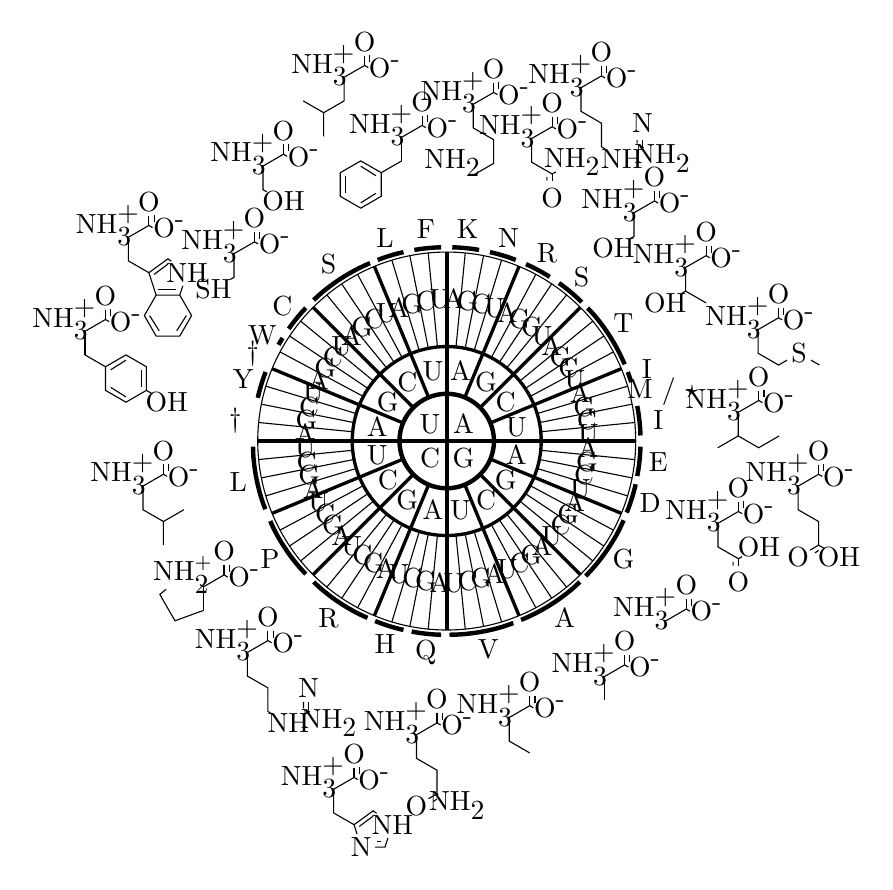
\begin{tikzpicture}[scale=.6]
		\tikzstyle{every node}=[inner sep=1.7pt,anchor=center]
		%	to_x and from_x styles denote bonds terminating or starting in labeled nodes. x denotes the number of letters in the node label.
		\tikzstyle{to_1}=[shorten >=5pt]
		\tikzstyle{to_1i}=[shorten >=6pt]
		\tikzstyle{to_2}=[shorten >=7pt]
		\tikzstyle{to_3}=[shorten >=8pt]
		\tikzstyle{from_1}=[shorten <=5pt]
		\tikzstyle{from_1i}=[shorten <=6pt]
		\tikzstyle{from_2}=[shorten <=8pt]
		\begin{scope}
		\draw [ultra thick] circle(1cm);
		\draw [ultra thick] (0:4)--(180:4) (90:4)--(270:4);
		\foreach \a/\l in {45/A,135/G,225/C,315/U}{
			\node at (90-\a:0.5cm) {\l};
		}
		\draw [very thick] circle(2cm);
		\foreach \A in {90,0,270,180}{
			\foreach \a/\l in {22.5/A,45/G,67.5/C,90/U}{
				\draw [very thick] (\A+\a:1) -- (\A+\a:4);
				\node at (\A-\a+11.25:1.5) {\l};
			}
		}
		\draw circle(4cm) (0:4)--(180:4) (90:4)--(270:4);
		\foreach \A in {90,180,270,0}{
			\foreach \a in {0,22.5,45,67.5}{
				\foreach \i/\l in {5.625/A,11.25/G,16.875/C,22.5/U}{
					\draw (\A+\a+\i:2) -- (\A+\a+\i:4);
					\node at (\A-\a-\i+2.8125:3) {\l};
				}
			}
		}
		\end{scope}
		\begin{scope}[scale=0.5]	% Lysine
		\draw[ultra thick,shorten >=2pt,shorten <=2pt] (90:8.2)
		arc(90:90-2*5.625:8.2);
		\path (90-0.8*5.625:14.3) node (zero) {};
		\draw[to_2]  (zero.center)	-- ++(30:1) node (CO) {}  
		-- +(330:1) node [anchor=base] {O$^{\mbox{-}}$};
		\draw[to_1]  (CO.center) 	-- +(90:1) node (Od) {O};
		\draw[to_1i] (CO.30)		-- +(90:1);
		\draw[to_3]  (zero.center)	-- ++(150:1) node {NH$_{\mbox{3}}^{\mbox{+}}$};
		\draw[to_3]  (zero.center)	-- ++(270:1) node(Cb){}
		-- ++(330:1) node (Cc) {}
		-- ++(270:1) node (Cd) {}
		-- ++(210:1) node (Ce) {}
		-- ++(150:1) node (Cf) {NH$_{\mbox{2}}$};
		\end{scope}
		\begin{scope}[scale=0.5]	% Asparagine
		\draw[ultra thick,shorten >=2pt,shorten <=2pt] (90-2*5.625:8.2)
		arc(90-2*5.625:90-4*5.625:8.2);
		\path (90-3.5*3.625-3:13.3) node (zero) {};
		\draw[to_2]  (zero.center)	-- ++(30:1) node (CO) {} 
		-- +(330:1) node [anchor=base] {O$^{\mbox{-}}$};
		\draw[to_1]  (CO.center)	-- +(90:1) node (Od) {O};
		\draw[to_1i] (CO.30)		-- +(90:1);
		\draw[to_3]  (zero.center)	-- ++(150:1) node {NH$_{\mbox{3}}^{\mbox{+}}$};
		\draw[to_2]  (zero.center)	-- ++(270:1) node(Cb){}
		-- ++(330:1) node (Cc) {}
		-- +(30:1) node (Cd) {NH$_{\mbox{2}}$};
		\draw[to_1i] (Cc.center)	-- +(270:1) node (O) {};
		\draw[to_1]  (Cc.210)		-- (O.150);
		\path (O.center) node {O};
		\end{scope}
		\begin{scope}[scale=0.5]	% Arginine
		\draw[ultra thick,shorten >=2pt,shorten <=2pt] (90-22.5:8.2)
		arc(90-22.5:90-33.75:8.2);
		\path (90-3.7*5.625:16) node (zero) {};
		\draw[to_2]  (zero.center)	-- ++(30:1) node (CO) {}
		-- +(330:1) node [anchor=base] {O$^{\mbox{-}}$};
		\draw[to_1]  (CO.center)	-- +(90:1) node (Od) {O};
		\draw[to_1i] (CO.30)		-- +(90:1);
		\draw[to_3]  (zero.center)	-- ++(150:1) node {NH$_{\mbox{3}}^{\mbox{+}}$};
		\draw[to_2]  (zero.center)	-- ++(270:1) node(Cb){}
		-- ++(330:1) node (Cc) {}
		-- ++(270:1) node (Cd) {}
		-- ++(330:1) node (NH1) {NH};
		\draw[from_2,to_3]  (NH1.center)	-- ++(30:1) node (Ce) {}
		-- ++(330:1) node {NH$_{\mbox{2}}$};
		\draw[to_1i] (Ce.center)	-- ++(90:1) node (N2) {};
		\draw[to_1]  (Ce.150)		-- (N2.210);
		\path (N2) node {N};
		\end{scope}
		\begin{scope}[scale=0.5]	% Serine
		\draw[ultra thick,shorten >=1pt,shorten <=2pt] (90-22.5-2*5.625:8.2)
		arc(90-33.75:90-33.75-11.25:8.2);
		\path (90-7*5.625:12.5) node (zero) {};
		\draw[to_2]  (zero.center)	-- ++(30:1) node (CO) {}
		-- +(330:1) node [anchor=base] {O$^{\mbox{-}}$};
		\draw[to_1]  (CO.center)	-- +(90:1) node (Od) {O};
		\draw[to_1i] (CO.30)		-- +(90:1);
		\draw[to_3]  (zero.center)	-- ++(150:1) node {NH$_{\mbox{3}}^{\mbox{+}}$};
		\draw[to_2]  (zero.center)	-- ++(270:1) node(Cb){} -- ++(210:1) node (Cc) {OH};
		\end{scope}
		\begin{scope}[scale=0.5]	% Threonine
		\draw[ultra thick,shorten >=1pt,shorten <=2pt] (90-45:8.2)
		arc(90-45:90-67.5:8.2);
		\path (90-45-0.8*11.25:12.5) node (zero) {};
		\draw[to_2]  (zero.center)	-- ++(30:1) node (CO) {}
		-- +(330:1) node [anchor=base] {O$^{\mbox{-}}$};
		\draw[to_1]  (CO.center)	-- +(90:1) node (Od) {O};
		\draw[to_1i] (CO.30)		-- +(90:1);
		\draw[to_3]  (zero.center)	-- ++(150:1) node {NH$_{\mbox{3}}^{\mbox{+}}$};
		\draw[to_2]  (zero.center)	-- ++(270:1) node(Cb){}
		-- ++(330:1) node (Cc) {} (Cb.center)
		-- +(210:1) node {OH};
		\end{scope}
		\begin{scope}[scale=0.5]	% Methionine
		\draw[ultra thick,shorten >=1pt,shorten <=2pt] (90-67.5:8.2)
		arc(90-67.5:90-67.5-5.625:8.2);
		\path (90-67.5-0.5*5.625:14) node (zero) {};
		\draw[to_2]  (zero.center)	-- ++(30:1) node (CO) {}
		-- +(330:1) node [anchor=base] {O$^{\mbox{-}}$};
		\draw[to_1]  (CO.center)	-- +(90:1) node (Od) {O};
		\draw[to_1i] (CO.30)		-- +(90:1);
		\draw[to_3]  (zero.center)	-- ++(150:1) node {NH$_{\mbox{3}}^{\mbox{+}}$};
		\draw[to_1]  (zero.center)	-- ++(270:1) node(Cb){}
		-- ++(330:1) node (Cc) {}
		-- ++(30:1) node (Cd) {S};
		\draw[from_1] (Cd.center)	-- +(330:1);
		\end{scope}
		\begin{scope}[scale=0.5]	% Isoleucine
		\draw[ultra thick,shorten >=1pt,shorten <=2pt] (0:8.2)
		arc(0:11.25:8.2);
		\path (1.0*5.625:12.4) node (zero) {};
		\draw[to_2]  (zero.center)	-- ++(30:1) node (CO) {}
		-- +(330:1) node [anchor=base] {O$^{\mbox{-}}$};
		\draw[to_1]  (CO.center)	-- +(90:1) node (Od) {O};
		\draw[to_1i] (CO.30)		-- +(90:1);
		\draw[to_3]  (zero.center)	-- ++(150:1) node {NH$_{\mbox{3}}^{\mbox{+}}$};
		\draw	     (zero.center)	-- ++(270:1) node(Cb){}
		-- ++(330:1) node (Cc) {}
		-- +(30:1) node (Cd) {} (Cb.center)
		-- +(210:1) node (Ce) {};
		\end{scope}
		\begin{scope}[scale=0.5]	% Glutamic acid
		\draw[ultra thick,shorten >=1pt,shorten <=2pt] (0:8.2)
		arc(0:-11.25:8.2);
		\path (-1.3*5.625:15) node (zero) {};
		\draw[to_2]  (zero.center)	-- ++(30:1) node (CO) {}
		-- +(330:1) node [anchor=base] {O$^{\mbox{-}}$};
		\draw[to_1]  (CO.center)  	-- +(90:1) node (Od) {O};
		\draw[to_1i] (CO.30)  		-- +(90:1);
		\draw[to_3]  (zero.center) 	-- ++(150:1) node {NH$_{\mbox{3}}^{\mbox{+}}$};
		\draw[to_1i] (zero.center) 	-- ++(270:1) node(Cb){} 
		-- ++(330:1) node (Cc) {} 
		-- ++(270:1) node (Cd) {}
		-- ++(330:1) node (NH) {OH};
		\draw[to_1]  (Cd.center) 	-- +(210:1) node (O) {};
		\draw[to_1i] (Cd.270) 		-- (O.300);
		\path (O.center) node {O};
		\end{scope}
		\begin{scope}[scale=0.5]	% Aspartic acid
		\draw[ultra thick,shorten >=1pt,shorten <=2pt] (-11.25:8.2)
		arc(-11.25:-22.5:8.2);
		\path (-11.25-5.625:12) node (zero) {};
		\draw[to_2]  (zero.center)	-- ++(30:1) node (CO) {}
		-- +(330:1) node [anchor=base] {O$^{\mbox{-}}$};
		\draw[to_1]  (CO.center) 	-- +(90:1) node (Od) {O};
		\draw[to_1i] (CO.30)		-- +(90:1);
		\draw[to_3]  (zero.center)	-- ++(150:1) node {NH$_{\mbox{3}}^{\mbox{+}}$};
		\draw[to_2]  (zero.center)	-- ++(270:1) node(Cb){}
		-- ++(330:1) node (Cc) {}
		-- +(30:1) node (Cd) {OH};
		\draw[to_1i] (Cc.center)	-- +(270:1) node (O) {};
		\draw[to_1]  (Cc.210)		-- (O.150);
		\path (O.center) node {O};
		\end{scope}
		\begin{scope}[scale=0.5]	% Glycine
		\draw[ultra thick,shorten >=1pt,shorten <=2pt] (-22.5:8.2)
		arc(-22.5:-45:8.2);
		\path (-33.75-1*5.625:12) node (zero) {};
		\draw[to_2]  (zero.center)	-- ++(30:1) node (CO) {}
		-- +(330:1) node [anchor=base] {O$^{\mbox{-}}$};
		\draw[to_1]  (CO.center)	-- +(90:1) node (Od) {O};
		\draw[to_1i] (CO.30)		-- +(90:1);
		\draw[to_3]  (zero.center)	-- ++(150:1) node {NH$_{\mbox{3}}^{\mbox{+}}$};
		\end{scope}
		\begin{scope}[scale=0.5]	% Alanine
		\draw[ultra thick,shorten >=1pt,shorten <=2pt] (-45:8.2)
		arc(-45:-68.25:8.2);
		\path (-45-11.25:12) node (zero) {};
		\draw[to_2]  (zero.center)	-- ++(30:1) node (CO) {}
		-- +(330:1) node [anchor=base] {O$^{\mbox{-}}$};
		\draw[to_1]  (CO.center)	-- +(90:1) node (Od) {O};
		\draw[to_1i] (CO.30)		-- +(90:1);
		\draw[to_3]  (zero.center)	-- ++(150:1) node {NH$_{\mbox{3}}^{\mbox{+}}$};
		\draw	     (zero.center)	-- ++(270:1) node(Cb){};
		\end{scope}
		\begin{scope}[scale=0.5]	% Valine
		\draw[ultra thick,shorten >=1pt,shorten <=2pt] (-68.25:8.2)
		arc(-68.25:-90:8.2);
		\path (-68.25-0.8*11.25:12) node (zero) {};
		\draw[to_2]  (zero.center)	-- ++(30:1) node (CO) {}
		-- +(330:1) node [anchor=base] {O$^{\mbox{-}}$};
		\draw[to_1]  (CO.center)	-- +(90:1) node (Od) {O};
		\draw[to_1i] (CO.30)		-- +(90:1);
		\draw[to_3]  (zero.center)	-- ++(150:1) node {NH$_{\mbox{3}}^{\mbox{+}}$};
		\draw (zero.center)		-- ++(270:1) node(Cb){}
		-- ++(330:1) node (Cc) {};
		\end{scope}
		\begin{scope}[scale=0.5]	% Glutamine
		\draw[ultra thick,shorten >=1pt,shorten <=2pt] (-90:8.2)
		arc(-90:-101.25:8.2);
		\path (-90.25-5.625:12.5) node (zero) {};
		\draw[to_2]  (zero.center)	-- ++(30:1) node (CO) {}
		-- +(330:1) node [anchor=base] {O$^{\mbox{-}}$};
		\draw[to_1]  (CO.center)	-- +(90:1) node (Od) {O};
		\draw[to_1i] (CO.30)		-- +(90:1);
		\draw[to_2]  (zero.center)	-- ++(150:1) node {NH$_{\mbox{3}}^{\mbox{+}}$};
		\draw[to_3]  (zero.center)	-- ++(270:1) node(Cb){}
		-- ++(330:1) node (Cc) {}
		-- ++(270:1) node (Cd) {}
		-- ++(330:1) node (NH) {NH$_{\mbox{2}}$};
		\draw[to_1]  (Cd.center)	-- +(210:1) node (O) {};
		\draw[to_1i] (Cd.270)		-- (O.300);
		\path (O.center) node {O};
		\end{scope}
		\begin{scope}[scale=0.5]	% Histidine
		\draw[ultra thick,shorten >=1pt,shorten <=2pt] (-101.25:8.2)
		arc(-101.25:-101.25-11.25:8.2);
		\path (-101.25-1.2*5.625:15.5) node (zero) {};
		\draw[to_2]  (zero.center)	-- ++(30:1) node (CO) {}
		-- +(330:1) node [anchor=base] {O$^{\mbox{-}}$};
		\draw[to_1]  (CO.center)	-- +(90:1) node (Od) {O};
		\draw[to_1i] (CO.30)		-- +(90:1);
		\draw[to_3]  (zero.center)	-- ++(150:1) node {NH$_{\mbox{3}}^{\mbox{+}}$};
		\draw        (zero.center)	-- ++(270:1) node(Cb){}
		-- ++(330:1) node(Cc){};
		\draw[to_2]  (Cc.center)	-- ++(108-1*72:1) node (Cd) {}
		-- ++(108-2*72:1) node (Ce) {NH};
		\draw[from_1,to_1] (Ce.center)	-- ++(108-3*72:1) node (Cf) {}
		-- ++(108-4*72:1) node (Cg) {};
		\draw[from_1] (Cg.center)	-- (Cc.center);
		\draw         (Cc.198+2*72)	-- (Cd.198+1*72);
		\draw[from_1] (Cg.72)		-- (Cf.198+4*72);
		\draw (Cg.center) node {N};
		\end{scope}
		\begin{scope}[scale=0.5]	% Arginine
		\draw[ultra thick,shorten >=2pt,shorten <=2pt] (-90-22.5:8.2)
		arc(-90-22.5:-90-45:8.2);
		\path (-90-7.7*5.625:12.3) node (zero) {};
		\draw[to_2]  (zero.center)	-- ++(30:1) node (CO) {}
		-- +(330:1) node [anchor=base] {O$^{\mbox{-}}$};
		\draw[to_1]  (CO.center)	-- +(90:1) node (Od) {O};
		\draw[to_1i] (CO.30)		-- +(90:1);
		\draw[to_3]  (zero.center)	-- ++(150:1) node {NH$_{\mbox{3}}^{\mbox{+}}$};
		\draw[to_2]  (zero.center)	-- ++(270:1) node(Cb){}
		-- ++(330:1) node (Cc) {}
		-- ++(270:1) node (Cd) {}
		-- ++(330:1) node (NH1) {NH};
		\draw[from_1i,to_3] (NH1.center)-- ++(30:1) node (Ce) {}
		-- ++(330:1) node {NH$_{\mbox{2}}$};
		\draw[to_1]  (Ce.center)	-- ++(90:1) node (N2) {};
		\draw[shorten >=4pt] (Ce.150)	-- (N2.210);
		\path (N2) node {N};
		\end{scope}
		\begin{scope}[scale=0.5]	% Proline
		\draw[ultra thick,shorten >=2pt,shorten <=2pt] (-90-45:8.2)
		arc(-90-45:-90-45-22.25:8.2);
		\path (-90-10.5*5.625:12) node (zero) {};
		\draw[to_2]  (zero.center)	-- ++(30:1) node (CO) {}
		-- +(330:1) node [anchor=base] {O$^{\mbox{-}}$};
		\draw[to_1]  (CO.center)	-- +(90:1) node (Od) {O};
		\draw[to_1i] (CO.30)		-- +(90:1);
		\draw[to_2]  (zero.center)	-- ++(150:1) node (nh) {NH$_{\mbox{2}}^+$};
		\draw        (zero.center)	-- ++(270:1) node(Cb){};
		\path        (Cb.center)	-- +(150:1) node (x) {};
		\path        (x.center)  	+(170:1) node (Cd) {};
		\path        (x.center)  	+(250:1) node (Cc) {};
		\draw[to_3]  (Cb.center)	-- (Cc.center)
		-- (Cd.center)
		-- (nh.center);
		\end{scope}
		\begin{scope}[scale=0.5]	% Leucine
		\draw[ultra thick,shorten >=2pt,shorten <=2pt] (180:8.2)
		arc(180:180+22.25:8.2);
		\path (-90-14.5*5.625:13) node (zero) {};
		\draw[to_2]  (zero.center)	-- ++(30:1) node (CO) {}
		-- +(330:1) node [anchor=base] {O$^{\mbox{-}}$};
		\draw[to_1]  (CO.center)	-- +(90:1) node (Od) {O};
		\draw[to_1i] (CO.30)		-- +(90:1);
		\draw[to_3]  (zero.center)	-- ++(150:1) node {NH$_{\mbox{3}}^{\mbox{+}}$};
		\draw (zero.center)		-- ++(270:1) node(Cb){}
		-- ++(330:1) node (Cc) {}
		-- +(30:1) node (Cd) {} (Cc.center)
		-- +(270:1) node (Ce) {};
		\end{scope}
		\begin{scope}[scale=0.5]	% Tyrosine
		\draw[ultra thick,shorten >=2pt,shorten <=2pt] (180-11.25:8.2)
		arc(180-11.25:180-22.5:8.2);
		\path (180-3*5.625:16) node (zero) {};
		\draw[to_2]  (zero.center)	-- ++(30:1) node (CO) {}
		-- +(330:1) node [anchor=base] {O$^{\mbox{-}}$};
		\draw[to_1]  (CO.center)	-- +(90:1) node (Od) {O};
		\draw[to_1i] (CO.30)		-- +(90:1);
		\draw[to_3]  (zero.center)	-- ++(150:1) node {NH$_{\mbox{3}}^{\mbox{+}}$};
		\draw 	     (zero.center)	-- ++(270:1) node(Cb){};
		\draw	     (Cb.center)	-- ++(330:1) node (Cc) {}
		-- ++(30:1) node (Cd) {}
		-- ++(330:1) node (Ce) {}
		-- ++(270:1) node (Cf) {}
		-- ++(210:1) node (Cg) {}
		-- ++(150:1) node (Ch) {}
		-- ++(90:1);
		\draw        (Cc.330)		-- (Cd.270);
		\draw        (Ce.210)		-- (Cf.150);
		\draw        (Cg.90)		-- (Ch.30);
		\draw[to_1i] (Cf.center)	-- +(330:1) node (OH) {OH};
		\end{scope}
		\begin{scope}[scale=0.5]	% Tryptophane
		\draw[ultra thick,shorten >=2pt,shorten <=2pt] (180-22.5-5.625:8.2)
		arc(180-22.5-5.625:180-22.5-11.25:8.2);
		\path (180-22.5-1.8*5.625:16) node (zero) {};
		\draw[to_2]  (zero.center)	-- ++(30:1) node (CO) {}
		-- +(330:1) node [anchor=base] {O$^{\mbox{-}}$};
		\draw[to_1]  (CO.center)	-- +(90:1) node (Od) {O};
		\draw[to_1i] (CO.30)		-- +(90:1);
		\draw[to_3]  (zero.center)	-- ++(150:1) node {NH$_{\mbox{3}}^{\mbox{+}}$};
		\draw 	     (zero.center)	-- ++(270:1) node(Cb){}
		-- ++(330:1) node(Cc){};
		\draw[to_2]  (Cc.center)	-- ++(108-1*72:1) node (Cd) {}
		-- ++(108-2*72:1) node (Ce) {NH};
		\draw[from_1](Ce.center)	-- ++(108-3*72:1) node (Cf) {}
		-- ++(108-4*72:1) node (Cg) {};
		\draw 	     (Cg.center)	-- (Cc.center);
		\draw        (Cc.198+2*72)	-- (Cd.198+1*72);
		\draw 	     (Cg.72)		-- (Cf.198+4*72);
		\draw	     (Cg.center)	-- ++(240:1) node (Ch) {}
		-- ++(300:1) node (Ci) {}
		-- ++(0:1) node (Cj) {}
		-- ++(60:1) node (Ck) {}
		-- ++(120:1) node (Cl) {};
		\draw	     (Ch.0)		-- (Ci.60);
		\draw	     (Cj.120)		-- (Ck.180);
		\end{scope}
		\begin{scope}[scale=0.5]	% Cysteine
		\draw[ultra thick,shorten >=2pt,shorten <=2pt] (180-45+11.25:8.2)
		arc(180-45+11.25:180-45:8.2);
		\path (180-45+11.25-1*7.625:12) node (zero) {};
		\draw[to_2]  (zero.center)	-- ++(30:1) node (CO) {}
		-- +(330:1) node [anchor=base] {O$^{\mbox{-}}$};
		\draw[to_1]  (CO.center)	-- +(90:1) node (Od) {O};
		\draw[to_1i] (CO.30)		-- +(90:1);
		\draw[to_3]  (zero.center)	-- ++(150:1) node {NH$_{\mbox{3}}^{\mbox{+}}$};
		\draw[to_2]  (zero.center)	-- ++(270:1) node(Cb){}
		-- ++(210:1) node (Cc) {SH};
		\end{scope}
		\begin{scope}[scale=0.5]	% Serine
		\draw[ultra thick,shorten >=1pt,shorten <=2pt] (90+45:8.2)
		arc(90+45:90+45-22.5:8.2);
		\path (90+45-11.25+0*5.625:14) node (zero) {};
		\draw[to_2]  (zero.center)	-- ++(30:1) node (CO) {}
		-- +(330:1) node [anchor=base] {O$^{\mbox{-}}$};
		\draw[to_1]  (CO.center)	-- +(90:1) node (Od) {O};
		\draw[to_1i] (CO.30)		-- +(90:1);
		\draw[to_3]  (zero.center)	-- ++(150:1) node {NH$_{\mbox{3}}^{\mbox{+}}$};
		\draw[to_2]  (zero.center)	-- ++(270:1) node(Cb){}
		-- ++(330:1) node (Cc) {OH};
		\end{scope}
		\begin{scope}[scale=0.5]	% Leucine
		\draw[ultra thick,shorten >=2pt,shorten <=2pt] (90+22.5:8.2)
		arc(90+22.5:90+11.25:8.2);
		\path (90+22.5-1.2*5.625:16) node (zero) {};
		\draw[to_2]  (zero.center)	-- ++(30:1) node (CO) {}
		-- +(330:1) node [anchor=base] {O$^{\mbox{-}}$};
		\draw[to_1]  (CO.center)	-- +(90:1) node (Od) {O};
		\draw[to_1i] (CO.30)		-- +(90:1);
		\draw[to_3]  (zero.center)	-- ++(150:1) node {NH$_{\mbox{3}}^{\mbox{+}}$};
		\draw 	     (zero.center)	-- ++(270:1) node(Cb){}
		-- ++(210:1) node (Cc) {}
		-- +(150:1) node (Cd) {} (Cc.center)
		-- +(270:1) node (Ce) {};
		\end{scope}
		\begin{scope}[scale=0.5]	% Phenylalanine
		\draw[ultra thick,shorten >=2pt,shorten <=2pt] (90+11.25:8.2)
		arc(90+11.25:90:8.2);
		\path (90+1.5*5.625:13) node (zero) {};
		\draw[to_2]  (zero.center)	-- ++(30:1) node (CO) {}
		-- +(330:1) node [anchor=base] {O$^{\mbox{-}}$};
		\draw[to_1]  (CO.center)	-- +(90:1) node (Od) {O};
		\draw[to_1i] (CO.30)		-- +(90:1);
		\draw[to_3]  (zero.center)	-- ++(150:1) node {NH$_{\mbox{3}}^{\mbox{+}}$};
		\draw	     (zero.center)	-- ++(270:1) node(Cb){};
		\draw	     (Cb.center)	-- ++(210:1) node (Cc) {}
		-- ++(150:1) node (Cd) {}
		-- ++(210:1) node (Ce) {}
		-- ++(270:1) node (Cf) {}
		-- ++(330:1) node (Cg) {}
		-- ++(30:1) node (Ch) {}
		-- ++(90:1);
		\draw	     (Cc.210)		-- (Cd.270);
		\draw	     (Ce.330)		-- (Cf.30);
		\draw	     (Cg.90)		-- (Ch.150);
		\end{scope}
		\node at (90-1*5.625:4.5) {K};
		\node at (90-3*5.625:4.5) {N};
		\node at (90-5*5.625:4.5) {R};
		\node at (90-7*5.625:4.5) {S};
		\node at (90-10*5.625:4.5) {T};
		\node at (90-12.5*5.625:4.5) {I};
		\node at (90-13.7*5.625:4.7) {M / $\star$};
		\node at (90-15*5.625:4.5) {I};
		\node at (90-17*5.625:4.5) {E};
		\node at (90-19*5.625:4.5) {D};
		\node at (90-22*5.625:4.5) {G};
		\node at (90-26*5.625:4.5) {A};
		\node at (90-30*5.625:4.5) {V};
		\node at (90-33*5.625:4.5) {Q};
		\node at (90-35*5.625:4.5) {H};
		\node at (90-38*5.625:4.5) {R};
		\node at (90-42*5.625:4.5) {P};
		\node at (90-46*5.625:4.5) {L};
		\node at (90-49*5.625:4.5) {$\dagger$};
		\node at (90-51*5.625:4.5) {Y};
		\node at (90-52.3*5.625:4.5) {$\dagger$};
		\node at (90-53.3*5.625:4.5) {W};
		\node at (90-55*5.625:4.5) {C};
		\node at (90-58*5.625:4.5) {S};
		\node at (90-61*5.625:4.5) {L};
		\node at (90-63*5.625:4.5) {F};
		\end{tikzpicture}
	\end{center}
\end{frame}

\begin{frame}[fragile]{Start from the beginning...}
	\begin{verbatim}
	\begin{tikzpicture}
	\draw (0,0) -- (1,1);
	\end{tikzpicture}
	\end{verbatim}
	\begin{itemize}
		\item Draws the line:
	\end{itemize}
	\begin{tikzpicture}
	\draw (0,0) -- (1,1);
	\end{tikzpicture}
\end{frame}

\begin{frame}[fragile]{Coordinates}
	\begin{itemize}
		\item Default coordinates are centimeters. The first element in \texttt{(0,0)} is the $x-axis$, the second is the $y-axis$:
	\end{itemize}
	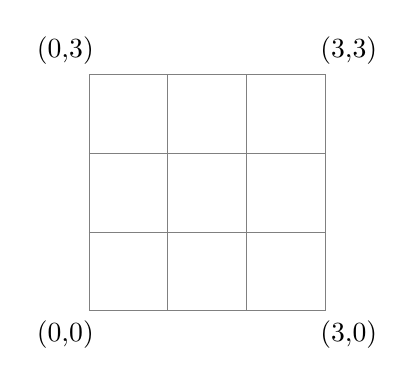
\begin{tikzpicture}
	\draw[help lines] (0,0) grid (3,3);
	\node[] at (-.3,-.3) {(0,0)};
	\node[] at (-.3,3.3) {(0,3)};
	\node[] at (3.3,-.3) {(3,0)};
	\node[] at (3.3,3.3) {(3,3)};
	\end{tikzpicture}
\end{frame}

\begin{frame}[fragile]{Nodes}
	\begin{itemize}
		\item TikZ pictures are structured around \textit{nodes}.
		\item Use them to place text, shapes, or to tell TikZ where to start and end an arrow.
		\item Drawing a circle and a rectangle nodes with text:
	\end{itemize}
	\begin{verbatim}
	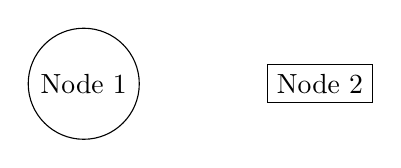
\begin{tikzpicture}
	\node[draw,circle] at (0,0) {Node 1};
	\node[draw,rectangle] at (3,0) {Node 2};
	\end{tikzpicture}
	\end{verbatim}
	
	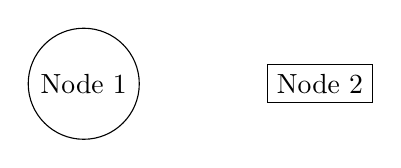
\begin{tikzpicture}
	\node[draw,circle] at (0,0) {Node 1};
	\node[draw,rectangle] at (3,0) {Node 2};
	\end{tikzpicture}
\end{frame}

\begin{frame}[fragile]{Unpacking}
	\begin{itemize}
		\item Each node is defined with \verb|\node|, and within [ ] we add options -- including the instruction to \cmd{draw} it.
		\item Text to be placed in the node comes at the end of the command line, inside \{\}.
		\item Each line of a tikz picture is one element (node, arrow, etc). Always end with a ``;''. Otherwise, you'll get an error when compiling.
		\item Use ``at'' for indicating the placement.
	\end{itemize}
\end{frame}

\begin{frame}[fragile]{Arrows}
	\begin{itemize}
		\item Arrow styles and heads are defined as options to \verb|\draw|:
	\end{itemize}
	\begin{verbatim}
	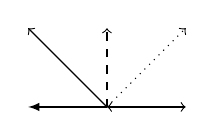
\begin{tikzpicture}
	\draw[->] (0,0) -- (-1,1);
	\draw[->,dashed] (0,0) -- (0,1);
	\draw[->,dotted] (0,0) -- (1,1);
	\draw[->,>=latex] (0,0) -- (-1,0);
	\draw[<->] (0,0) -- (1,0);
	\end{tikzpicture}
	\end{verbatim}
	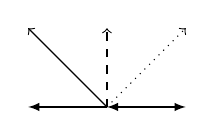
\begin{tikzpicture}
	\draw[->] (0,0) -- (-1,1);
	\draw[->,dashed] (0,0) -- (0,1);
	\draw[->,dotted] (0,0) -- (1,1);
	\draw[->,>=latex] (0,0) -- (-1,0);
	\draw[<->,>=latex] (0,0) -- (1,0);
	\end{tikzpicture}
\end{frame}

\begin{frame}[fragile]{Connecting Nodes}
	\begin{itemize}
		\item We can add labels to nodes, with a \texttt{(label)} right after closing the [ ] of \verb|\node| options:
		\item This way we refer to that node afterwards in the figure. 
		\item Note that to connect two nodes, the syntax for arrows is a bit different from the previous.
		\item The \cmd{above} option defines where the label will be in relation to the arrow. Can be also \cmd{below}, \cmd{left}, or \cmd{right}.
	\end{itemize}
	\begin{verbatim}
	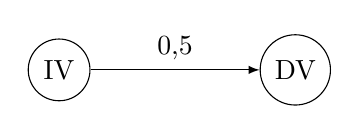
\begin{tikzpicture}
	\node[draw,circle] (x) at (0,0) {IV};
	\node[draw,circle] (y) at (3,0) {DV};
	\draw[->,>=latex,above] (x) to node {0,5} (y);
	\end{tikzpicture}
	\end{verbatim}
	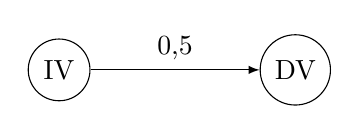
\begin{tikzpicture}
	\node[draw,circle] (x) at (0,0) {IV};
	\node[draw,circle] (y) at (3,0) {DV};
	\draw[->,>=latex,above] (x) to node {0,5} (y);
	\end{tikzpicture}
\end{frame}

\begin{frame}[fragile]{Paths and colors}
	\begin{itemize}
		\item If you specify multiple points for arrows, they'll form paths;
		\item Colors are passed as options to \verb|\draw|:
	\end{itemize}
	\begin{verbatim}
	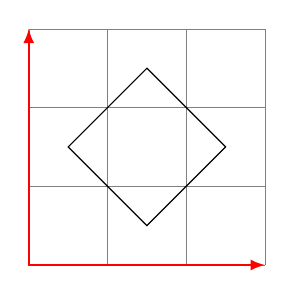
\begin{tikzpicture}
	\draw[help lines] (0,0) grid (3,3);
	\draw[<->,thick,red,>=latex] (0,3) -- (0,0) -- (3,0);
	\draw (1.5,0.5)--(2.5,1.5)--(1.5,2.5)--(0.5,1.5)--cycle;
	\end{tikzpicture}
	\end{verbatim}
	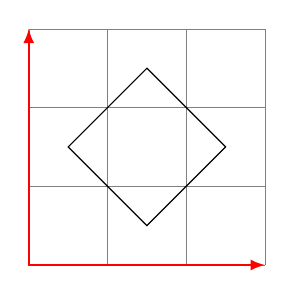
\begin{tikzpicture}
	\draw[help lines] (0,0) grid (3,3);
	\draw[<->,thick,red,>=latex] (0,3) -- (0,0) -- (3,0);
	\draw (1.5,0.5)--(2.5,1.5)--(1.5,2.5)--(0.5,1.5)--cycle;
	\end{tikzpicture}
\end{frame}

\begin{frame}[fragile]{Shapes}
	\begin{itemize}
		\item TikZ has built-in commands for simple shapes:
	\end{itemize}
	\begin{verbatim}
	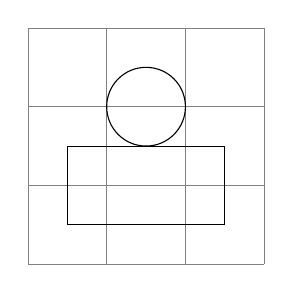
\begin{tikzpicture}
	\draw[help lines] (0,0) grid (3,3);
	\draw (1.5,2.0) circle (0.5);
	\draw (0.5,0.5) rectangle (2.5,1.5);
	\end{tikzpicture}
	\end{verbatim}
	
	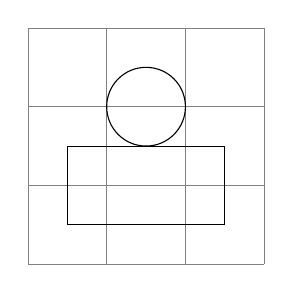
\begin{tikzpicture}
	\draw[help lines] (0,0) grid (3,3);
	\draw (1.5,2.0) circle (0.5);
	\draw (0.5,0.5) rectangle (2.5,1.5);
	\end{tikzpicture}
\end{frame}

\begin{frame}[fragile]{Shapes}
	\begin{itemize}
		\item The first coordinates in ( ) determine where the shape starts. In the case of the rectangle, it is the lower left corner. For the circle, it is the center.
		\item The second set of coordinates gives the size. The radius for circles, and the width and height for rectangles.
		\item Shapes, arrow styles, and several other features have to be loaded in the preamble as TikZ libraries:
	\end{itemize}
	\begin{verbatim}
	\usepackage{tikz}
	\usetikzlibrary{shapes,positioning,arrows}
	\end{verbatim} 
\end{frame}

\begin{frame}[fragile]{Positioning II}
	\begin{itemize}
		\item It is also practical to define the position of your first node, and all others in relation to that:
	\end{itemize}
	\begin{verbatim}
	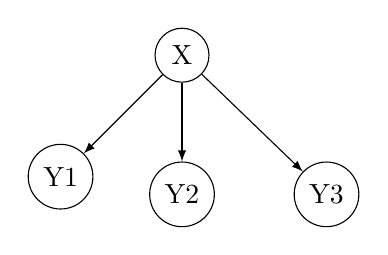
\begin{tikzpicture} 
		\node[draw,circle] (x) at (0,0) {X};
		\node[draw,circle] (y2) [below=of x] {Y2};
		\node[draw,circle] (y1) [below left=of x] {Y1};
		\node[draw,circle] (y3) [right=of y2] {Y3};
		\draw[->,>=latex] (x) -- (y1);
		\draw[->,>=latex] (x) -- (y2);
		\draw[->,>=latex] (x) -- (y3);
	\end{tikzpicture} 
	\end{verbatim}
	\begin{center} 
	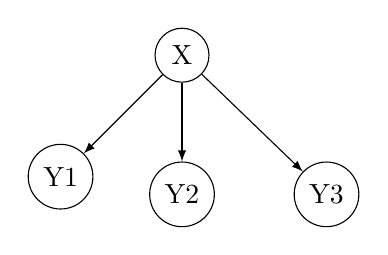
\begin{tikzpicture}
	\node[draw,circle] (x) at (0,0) {X};
	\node[draw,circle] (y2) [below=of x] {Y2};
	\node[draw,circle] (y1) [below left=of x] {Y1};
	\node[draw,circle] (y3) [right=of y2] {Y3};
	\draw[->,>=latex] (x) -- (y1);
	\draw[->,>=latex] (x) -- (y2);
	\draw[->,>=latex] (x) -- (y3);
	\end{tikzpicture}
	\end{center} 
\end{frame}

\begin{frame}[fragile]{Positioning II}
	\begin{itemize}
		\item Note that we can position a new node in relation to any other, \textit{as long as the other appears above it in the code!}
		\item Note the difference in position between Y1 and Y3 -- that's because Y1 is defined in relation to X, while Y3 is simply to the right of Y2.
		\item We can fix how far below (or above, to the right, etc) we want the new node. Replacing the Y3 line above with the following, for example:
	\end{itemize}
	\begin{verbatim}
	\node[draw,circle] (y3) [right= 5cm of y2] {Y3};
	\end{verbatim}
\end{frame}

\begin{frame}{Exercise}
\begin{itemize}
	\item Draw the following...
\end{itemize}
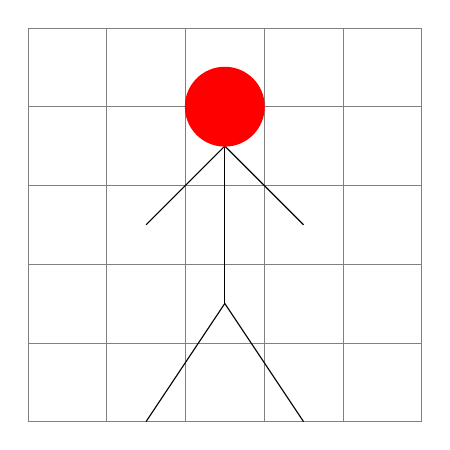
\begin{tikzpicture}
\draw[help lines] (0,0) grid (5,5);
\draw (1.5,0) -- (2.5,1.5);
\draw (3.5,0) -- (2.5,1.5);
\draw (2.5,1.5) -- (2.5,3.5);
\draw (2.5,3.5) -- (1.5,2.5);
\draw (2.5,3.5) -- (3.5,2.5);
\draw[fill,red] (2.5,4) circle (0.5);
\end{tikzpicture}
\end{frame}

\begin{frame}{Or, If You Want a Challenge...}
		\centering
		\footnotesize
		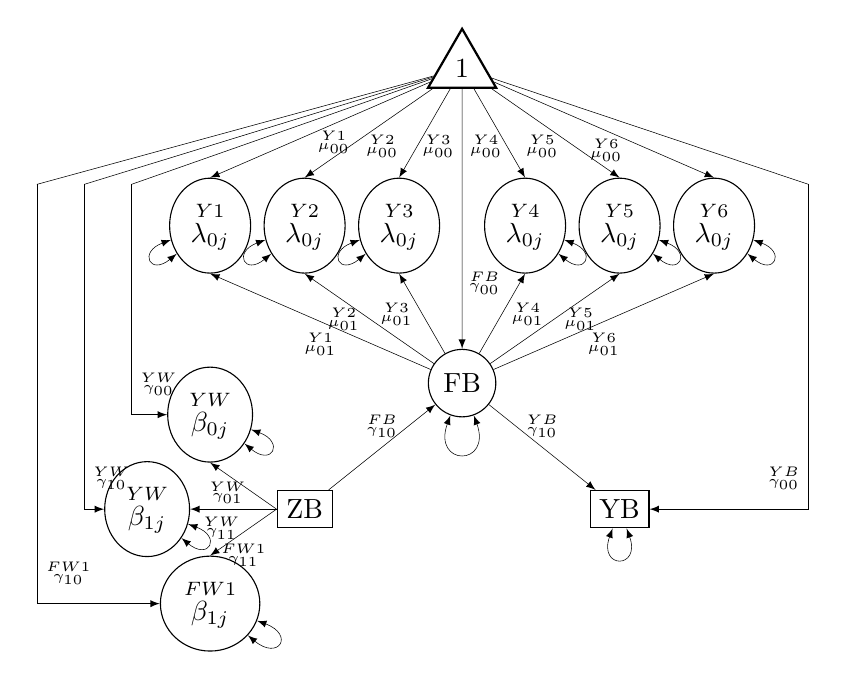
\begin{tikzpicture}[scale=.8]
		\node[draw,,regular polygon, regular polygon sides=3, inner sep=0pt, minimum size=1cm,thick] (inb) at (2.5, -5) {1};
		\node[draw,circle] (fb1) at (2.5,-10) {FB};
		\node[draw,ellipse] (y1b) at (-1.5,-7.5) {$\overset{Y1}{\lambda_{0j}}$};
		\node[draw,ellipse] (y2b) at (0,-7.5) {$\overset{Y2}{\lambda_{0j}}$};
		\node[draw,ellipse] (y3b) at (1.5,-7.5) {$\overset{Y3}{\lambda_{0j}}$};
		\node[draw,ellipse] (y4b) at (3.5,-7.5) {$\overset{Y4}{\lambda_{0j}}$};
		\node[draw,ellipse] (y5b) at (5,-7.5) {$\overset{Y5}{\lambda_{0j}}$};
		\node[draw,ellipse] (y6b) at (6.5,-7.5) {$\overset{Y6}{\lambda_{0j}}$};
		\node[draw,ellipse] (i1) at (-1.5,-10.5) {$\overset{YW}{\beta_{0j}}$};
		\node[draw,ellipse] (s1) at (-2.5,-12) {$\overset{YW}{\beta_{1j}}$};
		\node[draw,ellipse] (s2) at (-1.5,-13.5) {$\overset{FW1}{\beta_{1j}}$};
		\node[draw] (pb) at (0, -12) {ZB};
		\node[draw] (ob) at (5, -12) {YB};
		\draw [->, very thin, >=latex] (fb1)--(y1b.south) node [midway,below] {\tiny{$\overset{Y1}{\mu_{01}}$}};
		\draw [->, very thin, >=latex] (fb1)--(y2b.south) node [midway,left] {\tiny{$\overset{Y2}{\mu_{01}}$}};
		\draw [->, very thin, >=latex] (fb1)--(y3b.south) node [midway,left] {\tiny{$\overset{Y3}{\mu_{01}}$}};
		\draw [->, very thin, >=latex] (fb1)--(y4b.south) node [midway,right] {\tiny{$\overset{Y4}{\mu_{01}}$}};
		\draw [->, very thin, >=latex] (fb1)--(y5b.south) node [midway,right] {\tiny{$\overset{Y5}{\mu_{01}}$}};
		\draw [->, very thin, >=latex] (fb1)--(y6b.south) node [midway,below] {\tiny{$\overset{Y6}{\mu_{01}}$}};
		\draw [->, very thin, >=latex] (pb)--(fb1) node [midway, above] {\tiny$\overset{FB}{\gamma_{10}}$};
		\draw [->, very thin, >=latex] (fb1)--(ob) node [midway, above] {\tiny$\overset{YB}{\gamma_{10}}$};
		\draw [->, very thin, >=latex] (pb.west)--(i1.south) node [midway, below,yshift=2mm,xshift=-2mm] {\tiny$\overset{YW}{\gamma_{01}}$};
		\draw [->, very thin, >=latex] (pb.west)--(s1.east) node [midway, below,xshift=-1.5mm,yshift=0.5mm] {\tiny$\overset{YW}{\gamma_{11}}$};
		\draw [->, very thin, >=latex] (pb.west)--(s2.north) node [midway, below] {\tiny$\overset{FW1}{\gamma_{11}}$};
		\draw [->, very thin, >=latex] (inb)--(y1b.north) node  [midway,right,yshift=-1.5mm,xshift=-1.5mm] {\tiny$\overset{Y1}{\mu_{00}}$};
		\draw [->, very thin, >=latex] (inb)--(y2b.north) node  [midway,right,yshift=-1.5mm,xshift=-1.5mm] {\tiny$\overset{Y2}{\mu_{00}}$};
		\draw [->, very thin, >=latex] (inb)--(y3b.north) node  [midway,right,yshift=-1.5mm,xshift=-1.5mm] {\tiny$\overset{Y3}{\mu_{00}}$};
		\draw [->, very thin, >=latex] (inb)--(y4b.north) node  [midway,left,yshift=-1.5mm,xshift=1.5mm] {\tiny$\overset{Y4}{\mu_{00}}$};
		\draw [->, very thin, >=latex] (inb)--(y5b.north) node  [midway,left,yshift=-1.5mm,xshift=1.5mm] {\tiny$\overset{Y5}{\mu_{00}}$};
		\draw [->, very thin, >=latex] (inb)--(y6b.north) node  [midway,left,xshift=3.5mm,yshift=-2.5mm] {\tiny$\overset{Y6}{\mu_{00}}$};
		\draw [->, very thin, >=latex] (inb)--(fb1.north) node  [midway,right,xshift=-0.3mm,yshift=-8mm] {\tiny$\overset{FB}{\gamma_{00}}$};
		% arrows from intercept to beta0j^YW and beta0j^FW1:
		\node [draw=none] (coord1) at (-2.75, -7) {};
		\draw [-, very thin] (inb)--(coord1.north);
		\draw [->, very thin,>=latex] (coord1.north)|-(i1) node [midway, right,yshift=4mm] {\tiny$\overset{YW}{\gamma_{00}}$};
		\node [draw=none] (coord2) at (8 ,-7) {};
		\draw [-, very thin] (inb)--(coord2.north);
		\draw [->,very thin,>=latex] (coord2.north)|-(ob) node [midway, left,yshift=4mm] {\tiny$\overset{YB}{\gamma_{00}}$};
		\node [draw=none] (coord3) at (-3.5, -7) {};
		\draw [-, very thin] (inb)--(coord3.north);
		\draw [->, very thin,>=latex] (coord3.north)|-(s1) node [midway, right,yshift=4mm] {\tiny$\overset{YW}{\gamma_{10}}$};
		\node [draw=none] (coord4) at (-4.25, -7) {};
		\draw [-, very thin] (inb)--(coord4.north);
		\draw [->, very thin,>=latex] (coord4.north)|-(s2) node [midway, right,yshift=4mm] {\tiny$\overset{FW1}{\gamma_{10}}$};
		% Residuals:
		\draw[<->, very thin, >=latex] (y1b) to [out=200,in=220,looseness=6] (y1b);
		\draw[<->, very thin, >=latex] (y2b) to [out=200,in=220,looseness=6] (y2b);
		\draw[<->, very thin, >=latex] (y3b) to [out=200,in=220,looseness=6] (y3b);
		\draw[<->, very thin, >=latex] (y4b) to [out=320,in=340,looseness=6] (y4b);
		\draw[<->, very thin, >=latex] (y5b) to [out=320,in=340,looseness=6] (y5b);
		\draw[<->, very thin, >=latex] (y6b) to [out=320,in=340,looseness=6] (y6b);
		\draw[<->, very thin, >=latex] (i1) to [out=320,in=340,looseness=6] (i1);
		\draw[<->, very thin, >=latex] (s1) to [out=320,in=340,looseness=6] (s1);
		\draw[<->, very thin, >=latex] (s2) to [out=320,in=340,looseness=6] (s2);
		\draw[<->, very thin, >=latex] (ob) to [out=250,in=290,looseness=8] (ob);
		\draw[<->, very thin, >=latex] (fb1) to [out=250,in=290,looseness=6] (fb1);
		\end{tikzpicture}
\end{frame}

\begin{frame}[fragile]{Beamer}
\begin{itemize}
\item The class used for presentations is \cmd{Beamer}:
\begin{itemize}
\item \verb|\documentclass{beamer}|
\end{itemize}
\item Each slide is created with the commands \verb|\begin{frame}| and \verb|\end{frame}|
\item In the preamble we add information about authorship and title:
\begin{itemize}
\item Again using the commands \verb|\title{}| and \verb|author{}|;
\end{itemize}
\item But now we print them with a call to \verb|\titlepage|
\end{itemize}
\end{frame}

\begin{frame}[fragile]{Minimal Working Example}
	\begin{verbatim}
\documentclass{beamer}
\author{Presenter}
\title{Introducing Beamer}
\institute{Beaver University}
\begin{document}
\begin{frame}
\titlepage
\end{frame } % In practice, delete the space after frame
\end{document}
	\end{verbatim}
\end{frame}

\begin{frame}[fragile]{Themes}
\begin{itemize}
\item There are several \cmd{themes} that can be used to change the visual of beamer presentations.
\item Check a list at: \href{http://deic.uab.es/~iblanes/beamer_gallery/}{http://deic.uab.es/\textasciitilde iblanes/beamer\_gallery/}
\item They can be combined with different colors:
\end{itemize}
\begin{verbatim}
\documentclass{beamer}
\usetheme{Copenhagen}
\usecolortheme{beaver}
\end{verbatim}
\begin{itemize}
\item These commands go on the preamble.
\end{itemize}
\end{frame} 

\begin{frame}[fragile]{Other options in the preamble}
\begin{itemize}
\item A logo, included as a figure to be placed on the bottom right:
\begin{itemize}
\item \verb|logo{\includegraphics{...}}|
\end{itemize}
\item A subtitle to the presentation, with \verb|\subtitle{}|
\item An \verb|\inst{}| command, to add affiliation as footnotes:
\begin{itemize}
\item \verb|\author{Author One\inst{1} \and Author Two\inst{2}}|
\end{itemize}
\end{itemize}
\end{frame}


\begin{frame}[fragile]{Items}
\begin{itemize}
\item We use the \cmd{itemize} environment to create the bullet-points and indentation.
\item To send an item to the right, open another \cmd{itemize} environment inside the first.
\item You can have up to three nested \cmd{itemize}.
\end{itemize}
\begin{verbatim}
\begin{frame}{Frame Title}
\begin{itemize}
	\item First level
\begin{itemize}
		\item Second Level
\begin{itemize}
			\item Third Level
\end{itemize}
\end{itemize}
\end{itemize}
\end{verbatim}
\end{frame}

\begin{frame}[fragile]{Effects}
\begin{itemize}
\item To make items appear sequentially, use the \verb|\pause| command:
\end{itemize}
\begin{verbatim}
\begin{frame}
\begin{itemize} 
\item First thing \pause
\item Second thing
\end{itemize}
\end{verbatim}
\begin{itemize}
\item \LaTeX~will create two frames in the PDF output.
\end{itemize}
\end{frame} 

\begin{frame}[fragile]{Sections}
\begin{itemize}
\item We can also have sections in the presentation. Just use \verb|section{}| outside of a frame.
\item It's possible then to generate a Table of contents
\begin{itemize}
\item with the \verb|\tableofcontents| command.
\end{itemize}
\end{itemize} 
\end{frame} 

\begin{frame}[fragile]{Two-columns}
\begin{itemize}
\item To have two column slides, use the \cmd{columns} environment:
\end{itemize}
\begin{verbatim}
\begin{frame}
\begin{columns}
\column{.5\textwidth}
This is the first column

\column{.5\textwidth}
\begin{itemize}
\item This is the second column
\end{itemize}
\end{columns} 
\end{verbatim}
\end{frame}

\begin{frame}{Beamer Exercise}
\begin{itemize}
\item In Sharelatex there's a file called ``beamer\_exercise.tex''. It has the beginning to reproduce the file ``beamer\_exercise'' from the e-learning page.
\end{itemize}
\end{frame}

\begin{frame}{Final Practice}
	\begin{itemize}
		\item Two options:
		\begin{itemize}
			\item Choose a paper you've written, preferably with tables and graphs, and put it into \LaTeX.
			\item Or, format the last exercise file into \LaTeX.
		\end{itemize}
	\end{itemize}
\end{frame}



\end{document}
